\documentclass[11pt]{standalone}
\usepackage{amssymb}
\usepackage{amsmath}
\usepackage[no-math]{fontspec}
\usepackage{unicode-math}
\usepackage{libertinus}
\usepackage{pgf,xcolor}
\usepackage{tikz}
\usetikzlibrary{arrows.meta, backgrounds}
\usepackage{pgfplots}
\pgfplotsset{compat=newest}

\definecolor{my_darkgray}{HTML}{484949}
\definecolor{my_lightgray}{HTML}{F3F4F4}
\definecolor{my_darkblue}{HTML}{005A94}
\definecolor{my_lightblue}{HTML}{CCDEE9}
\definecolor{my_yellow}{HTML}{FFEC7F}
\definecolor{my_red}{HTML}{E60000}
\definecolor{my_orange}{HTML}{E87846}

\begin{document}
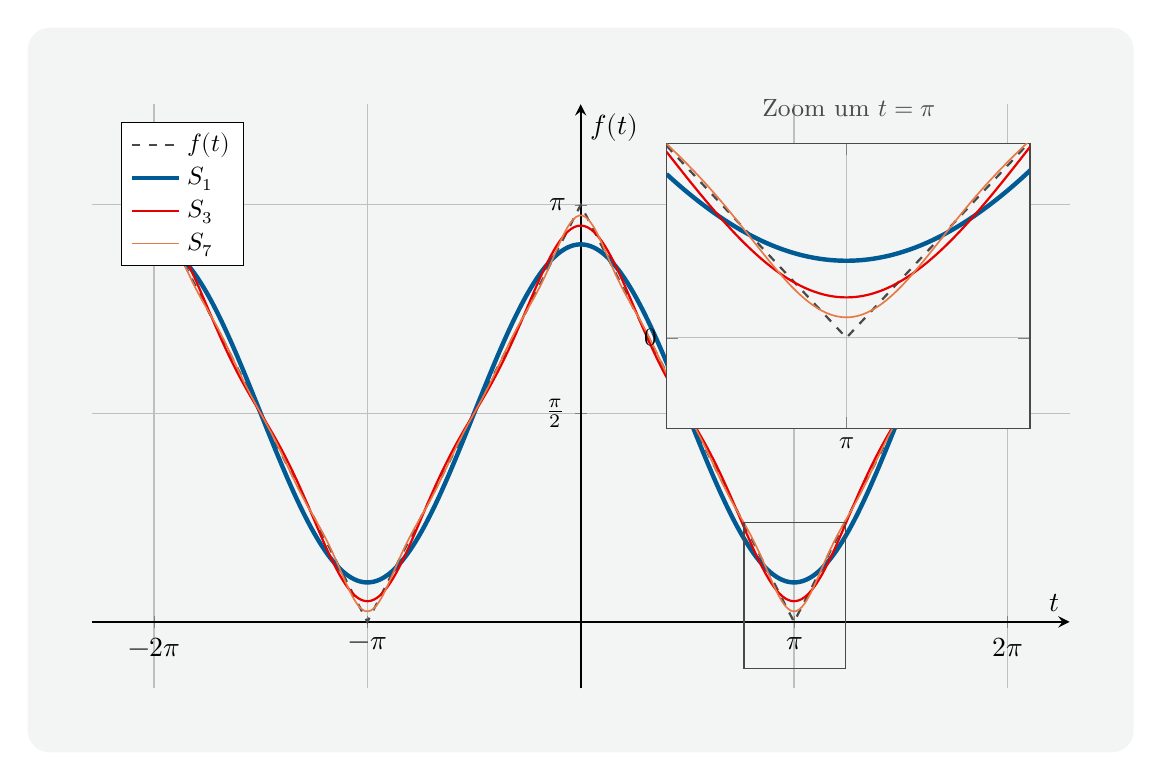
\begin{tikzpicture}[
    show background rectangle,
    background rectangle/.style={fill=my_lightgray, rounded corners=8pt},
    inner frame sep=0.8cm
]
\begin{axis}[
    name=main,
    axis lines = center,
    xlabel = {$t$},
    ylabel = {$f(t)$},
    grid = both,
    % axis equal hier bewusst weggelassen: Bei gleicher Skalierung wird die
    % Abbildung so flach gestaucht, dass die geringen Unterschiede zwischen
    % den Partialsummen nicht mehr erkennbar sind.
    axis line style={thick},
    width=14cm, height=9cm,
    xmin=-7.2, xmax=7.2,
    ymin=-0.5, ymax=3.9,
    xtick={-6.28319, -3.14159, 0, 3.14159, 6.28319},
    xticklabels={$-2\pi$, $-\pi$, $0$, $\pi$, $2\pi$},
    ytick={1.5708, 3.14159},
    yticklabels={$\tfrac{\pi}{2}$, $\pi$},
    legend pos=north west,
    legend style={font=\small},
    legend cell align=left,
]
% Exakte Dreiecksschwingung als Referenz (gestrichelt, sekundaer)
\addplot[draw=my_darkgray, thick, dashed] coordinates {
    (-6.28319, 3.14159)
    (-3.14159, 0)
    (0, 3.14159)
    (3.14159, 0)
    (6.28319, 3.14159)
};
\addlegendentry{$f(t)$}
% Partialsumme S_1: pi/2 + (4/pi) cos(t)
\addplot[draw=my_darkblue, samples=300, ultra thick, domain=-6.28319:6.28319]
    {pi/2 + (4/pi)*cos(deg(x))};
\addlegendentry{$S_1$}
% Partialsumme S_3: zusaetzlich (4/(9 pi)) cos(3t)
% Abnehmende Linienstaerken (S1 > S3 > S7), damit sich die fast
% deckungsgleichen Kurven gegenseitig nicht vollstaendig verdecken.
\addplot[draw=my_red, samples=300, thick, domain=-6.28319:6.28319]
    {pi/2 + (4/pi)*(cos(deg(x)) + cos(3*deg(x))/9)};
\addlegendentry{$S_3$}
% Partialsumme S_7: zusaetzlich Terme fuer n = 5 und n = 7
\addplot[draw=my_orange, samples=300, semithick, domain=-6.28319:6.28319]
    {pi/2 + (4/pi)*(cos(deg(x)) + cos(3*deg(x))/9
     + cos(5*deg(x))/25 + cos(7*deg(x))/49)};
\addlegendentry{$S_7$}
% Markierung des Zoom-Bereichs um die Knickstelle t = pi
\draw[my_darkgray, semithick]
    (axis cs:2.4, -0.35) rectangle (axis cs:3.9, 0.75);
\end{axis}
% Zoom-Ausschnitt um die Knickstelle t = pi: Die Partialsummen runden die
% Spitze ab und naehern sich dem Minimum von oben, ohne Ueberschwingen
% (kein Gibbssches Phaenomen, da f stetig ist).
\begin{axis}[
    at={(main.north east)}, anchor=north east,
    xshift=-0.5cm, yshift=-0.5cm,
    width=6.2cm, height=5.2cm,
    axis lines = box,
    axis line style={semithick, my_darkgray},
    axis background/.style={fill=my_lightgray},
    grid = both,
    xmin=2.4, xmax=3.9,
    ymin=-0.35, ymax=0.75,
    xtick={3.14159},
    xticklabels={$\pi$},
    ytick={0},
    yticklabels={$0$},
    tick label style={font=\small},
    title={Zoom um $t = \pi$},
    title style={font=\small, color=my_darkgray},
]
\addplot[draw=my_darkgray, thick, dashed] coordinates {
    (2.4, 0.741593)
    (3.14159, 0)
    (3.9, 0.758407)
};
\addplot[draw=my_darkblue, samples=300, ultra thick, domain=2.4:3.9]
    {pi/2 + (4/pi)*cos(deg(x))};
\addplot[draw=my_red, samples=300, thick, domain=2.4:3.9]
    {pi/2 + (4/pi)*(cos(deg(x)) + cos(3*deg(x))/9)};
\addplot[draw=my_orange, samples=300, semithick, domain=2.4:3.9]
    {pi/2 + (4/pi)*(cos(deg(x)) + cos(3*deg(x))/9
     + cos(5*deg(x))/25 + cos(7*deg(x))/49)};
\end{axis}
\end{tikzpicture}
\end{document}
